	\chapter{Δικτύωση}
		Δικτύωση στα ηλεκτρονικά παιχνίδια έχουμε όταν περισσότεροι από ένας παίχτες σε διαφορετικές πλατφόρμες ή υπολογιστές, μοιράζονται και αλληλεπιδρούν στο ίδιο εικονικό περιβάλλον. Παίχτες σε διάφορα σημεία του πλανήτη θέλουν να μοιραστούν ένα εικονικό περιβάλλον σε πραγματικό χρόνο με σκοπό την συνεργασία ή την αντιπαλότητα. O κόσμος είναι ένα υπερσύνολο του offline κόσμου με επιπλέων στοιχεία κοινωνικοποίησης όπως η επικοινωνία μέσω μηνυμάτων ή φωνής.
		
		\subsection{Αλληλεπίδραση σε εικονικό περιβάλλον}	
		Ένας εικονικός κόσμος, περιλαμβάνει πολλές οντότητες οι  οποίες αλληλεπιδρούν μεταξύ τους μέσω των μηχανισμών, νόμων και κανόνων που διέπουν τον κόσμο. Παράδειγμα μηχανισμού είναι η προσομοίωση του φυσικού κόσμου, όπου οι οντότητες αναποκρίνονται σε νόμους της φυσικής.
		
	    Κατά την ενημέρωση του κόσμου, ο προσομοιωτής χρησιμοποιώντας  τους νόμους, τους κανόνες και τους μηχανισμούς που διέπουν τον κόσμο, παίρνει ως είσοδο τις οντότητες, τα ειδικά βάρη των ιδιοτήτων τους, την απόλυτη θέση τους στο σύστημα συντεταγμένων του κόσμου, και το χρονικό διάστημα της προσομοίωσης και αναλύει την προσομοίωση. Η ανάλυση της προσομοίωσης για να είναι επιτρεπτά ακριβής πρέπει να γίνεται περίπου 80-100 φορές το δευτερόλεπτο. [αναφορά σε πηγή]
		
		Στο τέλος της προσομοίωσης, η μηχανή γραφικών αποτυπώνει τον κόσμο στις εξόδους με αναφορές σε στατικά assets, σε αλγόριθμους παραγωγής δυναμικών assets για την αναπαράσταση του κόσμου.
	
		\subsection{Οι απαιτήσεις του υποσυστήματος δικτύωσης}	
		Με βάση το πρόβλημα καταλήγουμε στο παρακάτω διάγραμμα ακολουθίας \ref{fig:Network_Sequence_Diagram}.
		
		\begin{figure}[h]
			\centering
			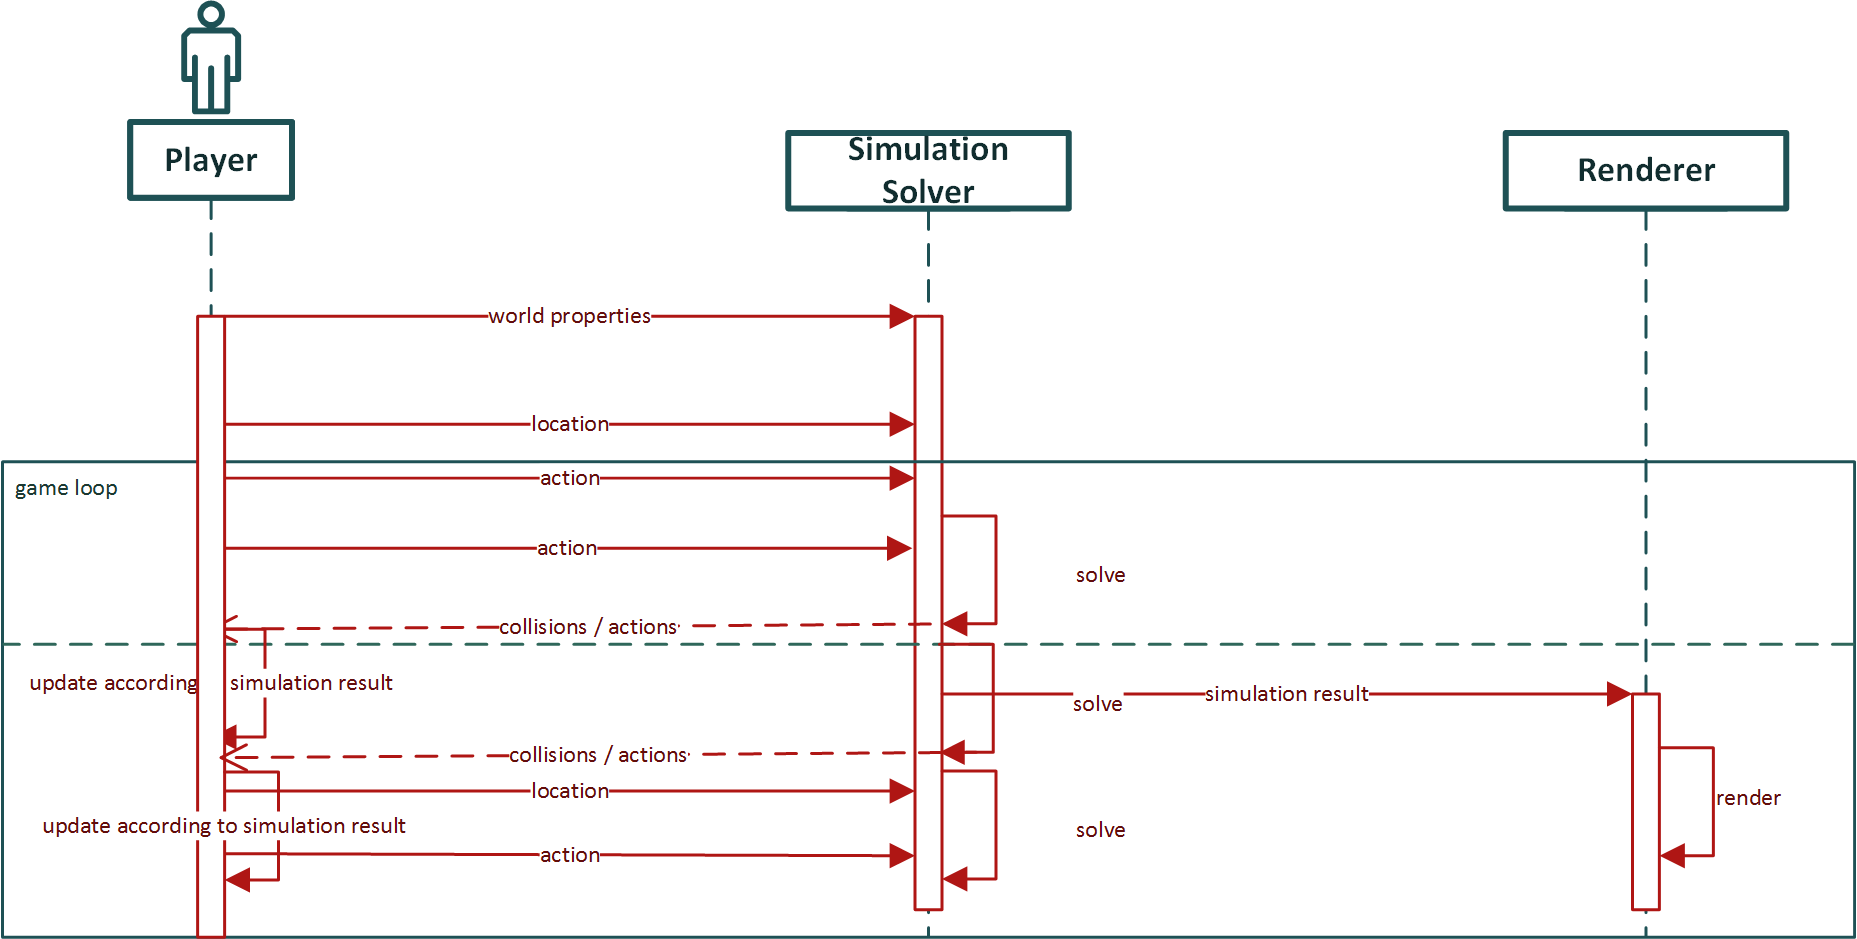
\includegraphics[width=140mm]{Images/gameloop_network_sequence}
			\caption{Network Sequence Diagram}
			\label{fig:Network_Sequence_Diagram}
		\end{figure}		
		
		Βλέποντας το διάγραμμα καταλαβαίνουμε ότι σε η διαδικασία rendering περιλαμβάνει στατικά στοιχεία και αλγόριθμους, τα οποίοι μπορούν να φορτώνονται τοπικά στον κάθε υπολογιστή, και δεν είναι απαραίτητα για την επίλυση της προσομοίωσης. Τα απαραίτητα στοιχεία για την προσομοίωση τα οποία πρέπει να μοιράζονται μεταξύ των παιχτών είναι:
		\begin{itemize}
			\item Oι ιδιότητες της οντότητας με βάση τους νόμους του κόσμου. Οι ιδιότητες αυτές δεν ενημερώνονται συχνά.
			\item Οι αλλαγές στο σύστημα συντεταγμένων και οι διάφορες ενέργειες της κατευθυνόμενης οντότητας κατά την πάροδο του χρόνου. Οι αλλαγές τοποθεσίας και ενέργειες γίνονται πολλές φορές ανά δευτερόλεπτο. Η προσομοίωση για να είναι ακριβής πρέπει να ενημερώνεται για τις διάφορες ενέργειες σε πραγματικό χρόνο.
		\end{itemize}
				
		\section{Ανάλυση εννοιών}	
		Η ανάγκη αποστολής πολλών μηνυμάτων ανά δευτερόλεπτο οδηγεί στη χρήση των network sockets. Τα sockets χρησιμοποιωντας ένα IP και  Port και επιτρέπουν την αποστολή και παραλαβή μηνυμάτων με βάση κάποιου πρωτόκολλου.
		
		\subsection{Πρωτοκόλο}
		\begin{itemize}	
			\item TCP (transmission control protocol), είναι το πιο συχνά χρησιμοποιημένο πρωτόκολλο. Η διασύνδεση με TCP είναι αξιόπιστη και τα μηνύματα παραλαμβάνονται στη σειρά αποστολής. Η αξιοπιστία όμως έρχεται με ένα μικρό κόστος απόδοσης.
			\item UDP Το UDP (user diagram protocol) δεν περιλαμβάνει την αξιοπιστία και την εγγύηση της αλληλουχίας μηνυμάτων. Η απουσία λειτουργιών όμως, το κάνει το πιο γρήγορο σε αποστολή μηνυμάτων πρωτόκολλο.
			
			Η επιλογή πρωτοκόλλου γίνεται ανάλογα με το γενικότερο πλαίσιο και τη συγκεκριμένη χρήση του πακέτου αποστολής. Στην αποστολή της τοποθεσίας, το οποίο γίνεται 20φορές / δευτερόλεπτο, η αξιοπιστία δεν είναι το βασικότερο, αλλά η απόδοση. Στην αποστολή των στοιχειών του χρήστη κατά την έναρξη, ή ενώς γραπτού μηνύματος πρέπει να είναι αξιόπιστη.
		\end{itemize}

		\subsection{Aρχιτεκτονική δικτύου}
			Οι αρχιτεκτονικές δικτύου χωρίζονται ανάλογα με το που γίνεται η επίλυση και επεξεργασία της προσομοίωσης.  
		\begin{itemize}	
			\item Client-server model: στο οποίο ο client απλά κάνει render και το μεγαλύτερο κομμάτι της λογικής και της προσωμοίωσης τρέχει στον server. Ο server στέλνει οδηγίες στον client για το τι να κάνει render και ο client απλά υπακούει.
			\item Client on top of server model: ο client είναι και server, δηλαδή οι μηχανές που έχουν τον client έχουν και τον server.
			\item Peer-to-peer: οι μηχανές συμπεριφέρονται μερικώς ως clients και μερικώς ως servers, δηλαδή έχουν και στοιχεία λογικής και επεξεργασίας.
		\end{itemize}
			Η client-server αρχιτεκτονική εφαρμόζεται σε παιχνίδια τα οποία περιλαμβάνουν πολύ μεγάλους κόσμους και η προσομοίωση περιλαμβάνει αλληλεπιδράσεις μεταξύ πολλών οντοτήτων. Οι προσωμοιώσεις αυτές γίνονται σε εξειδικευμένες μηχανές και όχι στον προσωπικό υπολογιστή του κάθε χρήστη γιατί χρειάζονται μεγάλους υπολογιστικούς πόρους. Επίσης ο server μπορεί να λύσει race conditions και να λειτουργήσει ως "διαιτητής" μεταξύ δύο οντοτήτων οι οποίες ζητούν πρόσβαση στο ίδιο σύστημα κατά το ίδιο χρονικό διάστημα. Οι αρχιτεκτονικές στις οποίες ο client περιλαμβάνει στοιχεία επεξεργασίας του κοινόχρηστου κόσμου, είναι πιο δύσκολες στην ανάπτυξη συντήρηση γιατί δημιουργούνται race conditions στο χρονικό διάστημα αποστολής-παραλαβής μηνυμάτων που προορίζονται σε αλληλοεξαρτώμενες λειτουργίες.
			
		\section{Σχεδίαση}
		Κατά το σχεδιασμό διαδικτυακών παιχνιδιών πολλά μοτίβα και στερεότυπα κώδικα επαναλαμβάνονται χωρίς να συμβάλλουν στην λογική ή μηχανισμούς. Σκοπός του framework είναι να μειώσει και να απλοποιήσει τον επαναλαμβανόμενο κώδικα και να προμηθεύσει τον χρήστη με μοτίβα και μοντέλα ούτως ώστε να εστιάσει μόνο στα απαραίτητα.
		
		\subsection{Οντότητες}
		\paragraph{Serialization}
		Σε μια αντικειμενοστραφή γλώσσα χρησιμοποιούνται κλάσεις για να μοντελοποιήσουν το πρόβλημα. Όμως τα αντικείμενα τον κλάσεων δεν μπορούν να σταλούν μέσω network socket στην αρχική τους μορφή, πρέπει να γίνει μια μετατροπή σε binary για να είναι συνεπής με το format των δεδομένων που αποστέλλονται μέσω του socket . Κατά την αποστολή έχουμε το serialization τον αντικείμενων, και κατά την παραλαβή το deserialization του πακέτου στο αντικείμενο που αντιπροσωπεύει.
		\subsection{Τύποι μηνυμάτων}
		Οι διάφοροι τύποι μηνυμάτων χρησιμοποιούνται για να ξεχωρίσουν την κατάσταση στην οποία βρίσκεται ο client ή ο server.
			\begin{itemize}
				\item Αλλαγή κατάστασης
				\begin{itemize}
					\item Connecting
					\item Connected
					\item Disconnecting
					\item Disconnected
				\end{itemize}
				\item Data
				\item ErrorMessage
				\item WarningMessage
				\item VerboseMessage
				\item ConnectionApproval
				\item DiscoveryRequest
				\item DiscoveryResponse
			\end{itemize}
		Οι τύποι μηνυμάτων μπορούν να μοντελοποιηθούν ως ένα enum και να προστεθεί η πληροφορία τους στο πρώτο byte του serialized μηνύματος. Το πρώτο byte του παραληφθέντα μηνύματος περιλαμβάνει τον τύπο του μηνύματος.
		
		\subsection{Διαχειριστής δικτύωσης}
		Ο διαχειριστής δικτύωσης (network manager) είναι υπεύθυνος για την διαχείριση των sockets, την αποστολή / παραλαβή μηνυμάτων, ενθυλακώνει λειτουργιες για την διαδικτύωση και είναι ο πηρύνας του framework και επεκτίνεται από τον client, server οι οποίοι προσθέτουν λειτουργίες.
			
		\section{Υλοποίηση}	
		\subsection{Τρόπος χρήσης}
		Η διαδικασία χρήσης \ref{fig:Network_Usage_Diagram} πρέπει να είναι εξορθολογιστική και ξεκάθαρη για εύκολη και γρήγορη ανάπτυξη και περιοριστική για αποφυγή bugs και προβληματων.
		\begin{figure}
			\centering
			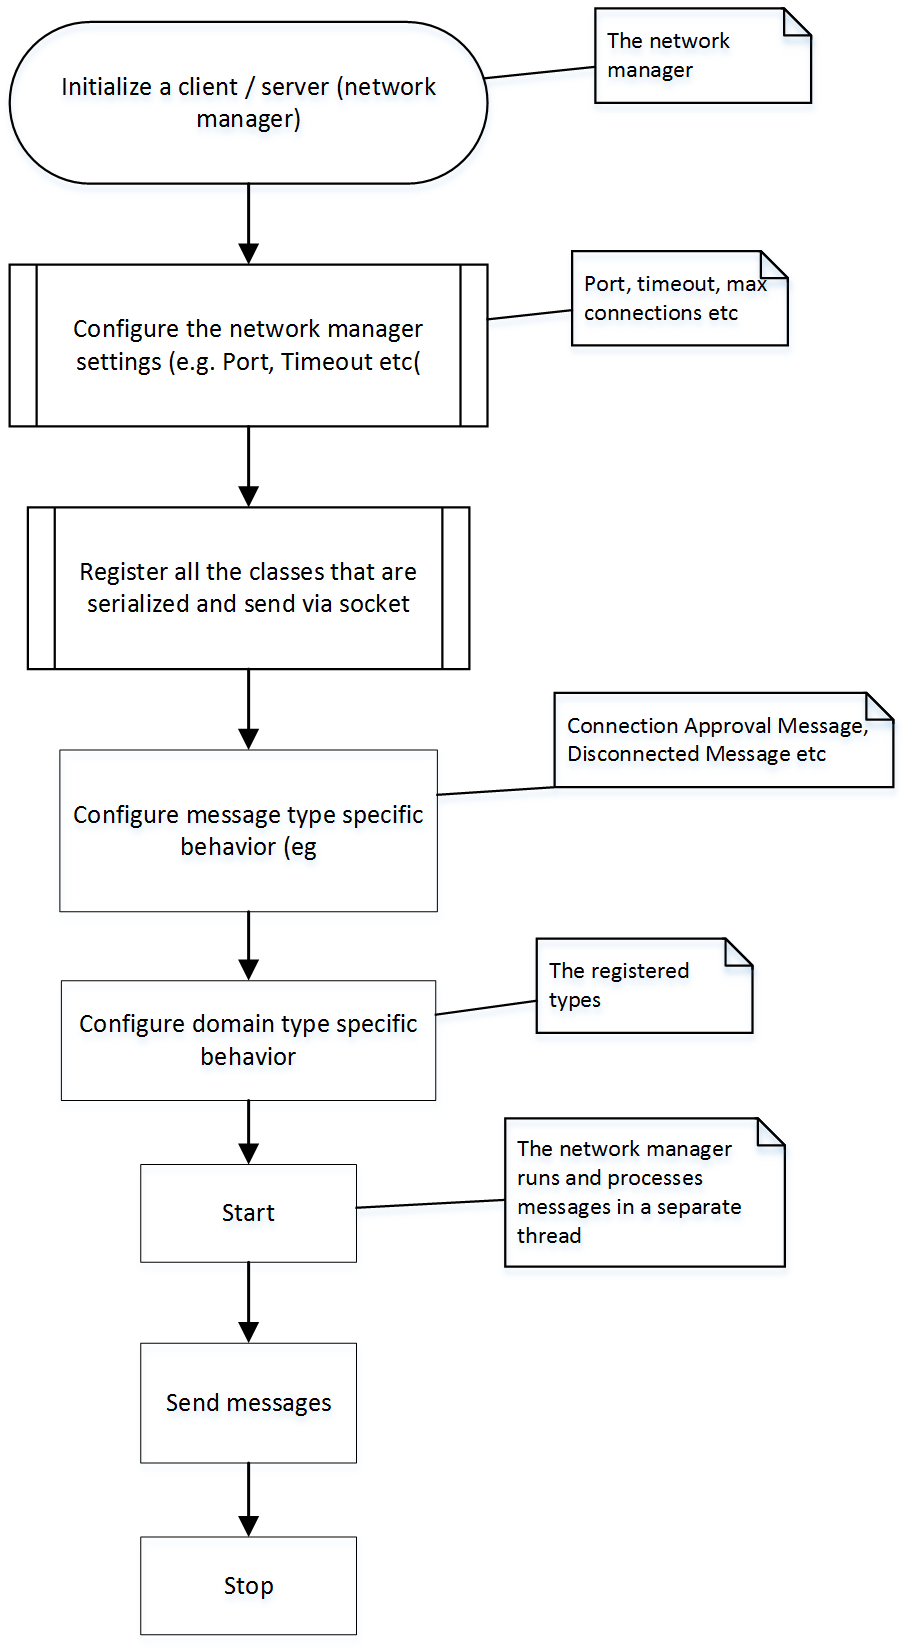
\includegraphics[width=100mm]{Images/network_usage_diagram}
			\caption{Network Usage Diagram}
			\label{fig:Network_Usage_Diagram}
		\end{figure}	
					
		\subsection{Αρχιτεκτονική}	
		Η αρχιτεκτονική στηρίζεται στην ανταλλαγή μηνυμάτων-κλάσεων και χωρίζεται στα παρακάτω επίπεδα.
			\begin{itemize}
				\item {Packages} Χειρίζεται το serialization, αναλύει τα εισερχόμενα μηνύματα και χειρίζεται τις ανακατευθύνσεις του εκτελούμενου κώδικα κατά την παραλαβή μηνυμάτων. 
				\item {Networking} Διαχειρίζεται τις συνδεσεις των χρηστών, τα sockets και ο,τι έχει να κάνει με διασύνδεση.
				\item {Auditing} Αφαιρετικό επίπεδο για logging. Ο χρήστης μπορεί να ενσωματώσει τη δική του λογική παρακολούθησης μηνυμάτων.
				\item{Infrastructure} Το επίπεδο αυτό περιέχει επαναχρησιμοποιήσημο κώδικα των πακέτων όπως το ConcurrentRepository, για thread-safe αποθήκευση κλειδιών και τιμών, και το ParallelBufferBlock το οποίο εκτελεί κώδικα σε buffer άλλου thread για ασύγχρονη επεξεργασία.
			\end{itemize}
			
			\subsection{Ανταλλαγή πακέτων}	 
			Το serialization των μηνυμάτων πρέπει να είναι ντερερμενιστικό ώστε να αναγνωρίζεται ο τύπος του μηνύματος και η κλάση την οποία αντιπροσωπεύει και ελαφρύς ώστε να μην επιβαρύνεται το network με επιπλέον δεδομένα. Ο ενσωματομένος serializer χρησιμοποιεί reflection για να αναγνωρίσει τα primitive properties της κλάσης. Για προχωριμένο serialization περίπλοκων τύπων, ο χρήστης έχει τη δυνατότητα να συμπεριλάβει τον δικό του serializer με το implementation του IPackageSerializer interface και την χωρήγηση του σημειώνοντας την κλάση με το PackageSerializerAttribute και τον τύπο του serializer.
			
			
			Κατά την προετοιμασία του network manager, o χρήστης καλείται να καταχωρίσει στο Container ποιες κλασεις θα χρησιμοποιηθούν κατά την ανταλλαγή μηνυμάτων. Οι κλάσεις που προωρίζονται για serialization σημειώνονται με κάποιο Attribute και η καταχώριση μπορεί να γίνει δυναμικά με reflection.
			Όταν τελειώσει η καταχώριση, το container χρησιμοποιώντας ένα ντετερμενιστικό αλγόριθμο ταξινομώντας με βάση το όνομα της κλάσης στο χώρο ονομάτων κτίζει ένα thread safe repository στο οποίο καταχωρείται ένα μοναδικό byte για αναγνωριστικό του κάθε τύπου και πληροφορίες για την χρήση του τύπου.
			
			Στο τέλος της καταχώρισης και της κατασκευής αλγόριθμου αντιστοίχισης αντικειμένων και λογικής, ο χρήστης μπορεί να καταχωρίσει εκτελέσημο κώδικα υπό μορφή function o οποίος εκτελείται ασύγχρονα κατά την παραλαβή κάποιου μηνύματος-κλάσης, τύπου μηνύματος, ή συμβάντος συγκεκριμένης σύνδεσης.
			
			Στο UML διάγραμμα \ref{network_packages} παρουσιάζεται το υποσύστημα διαχείρισης πακέτων.
			\begin{figure}
				\centering
				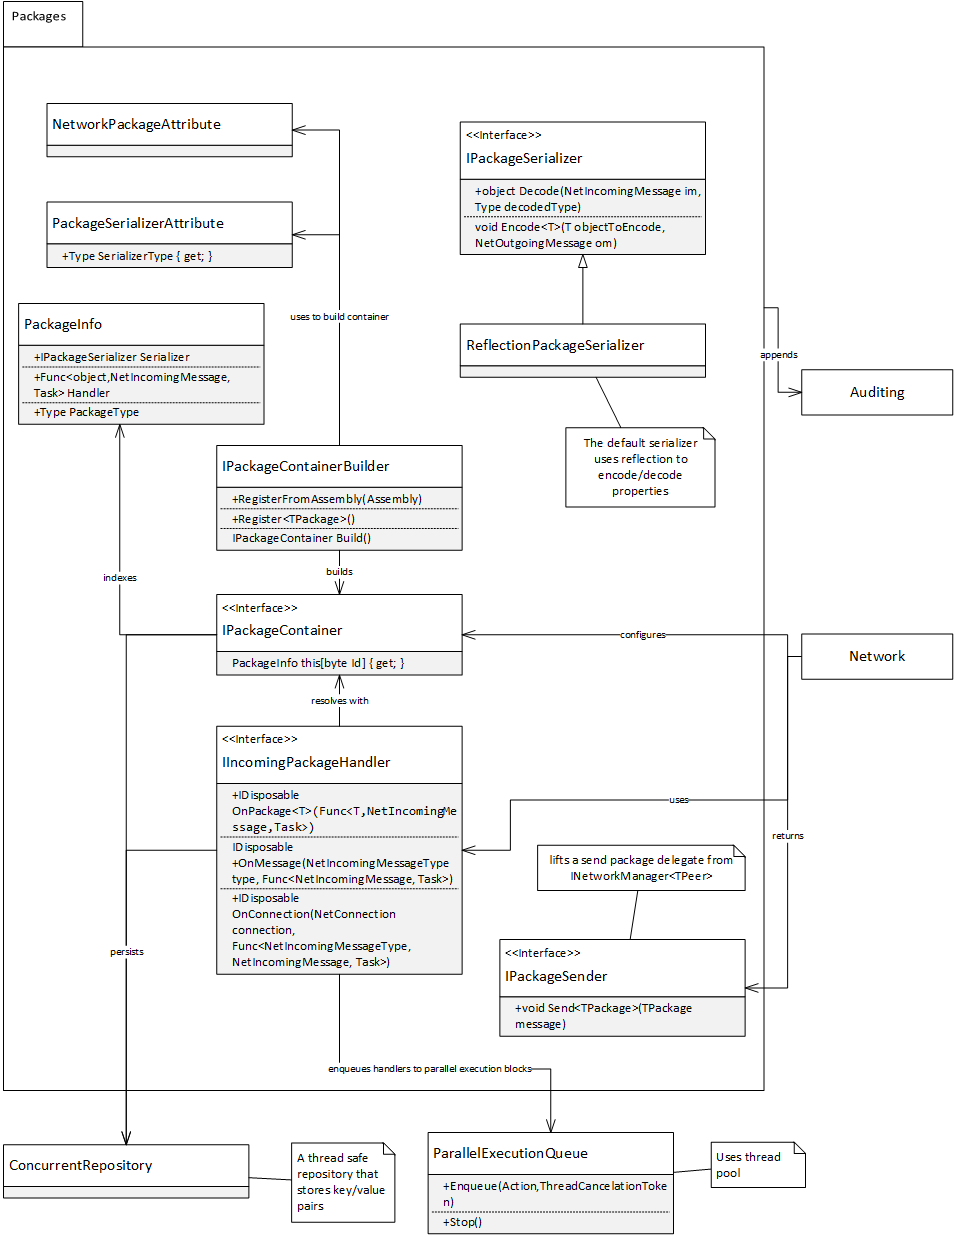
\includegraphics[width=165mm]{Images/network_architecture_packages}
				\caption{Network Packages Subsystem}
				\label{network_packages}
			\end{figure}	
					
			\subsection{Διαχείριση δικτύωσης}	 					
			
			Οι ρυθμίσεις του network manager κτίζονται από αφαιρέσεις. Η χρήση πρωτοκόλλων και τεχνικών γίνεται με άγνοια της υλοποίησης και λεπτομερειών.
			Η σχεδίαση επιτρέπει την αποστολή μηνύματος ανεξαρτήτου πρωτοκόλου, τρόπο αποστολής και παραλήπτη. Ο network manager περιλαμβάνει τεχνικές function lifting για αποστολή μηνυμάτων. Ο χρήστης μπορεί να ρυθμίσει διάφορους τρόπους αποστολής ανάλογα με το περιβάλλον χρήση, και να τους κρύψει πίσω από functions. Η αρχιτεκτονική του networking module παρουσιάζεται στο uml διάγραμμα \ref{networking_module}
						
			\begin{figure}
				\centering
				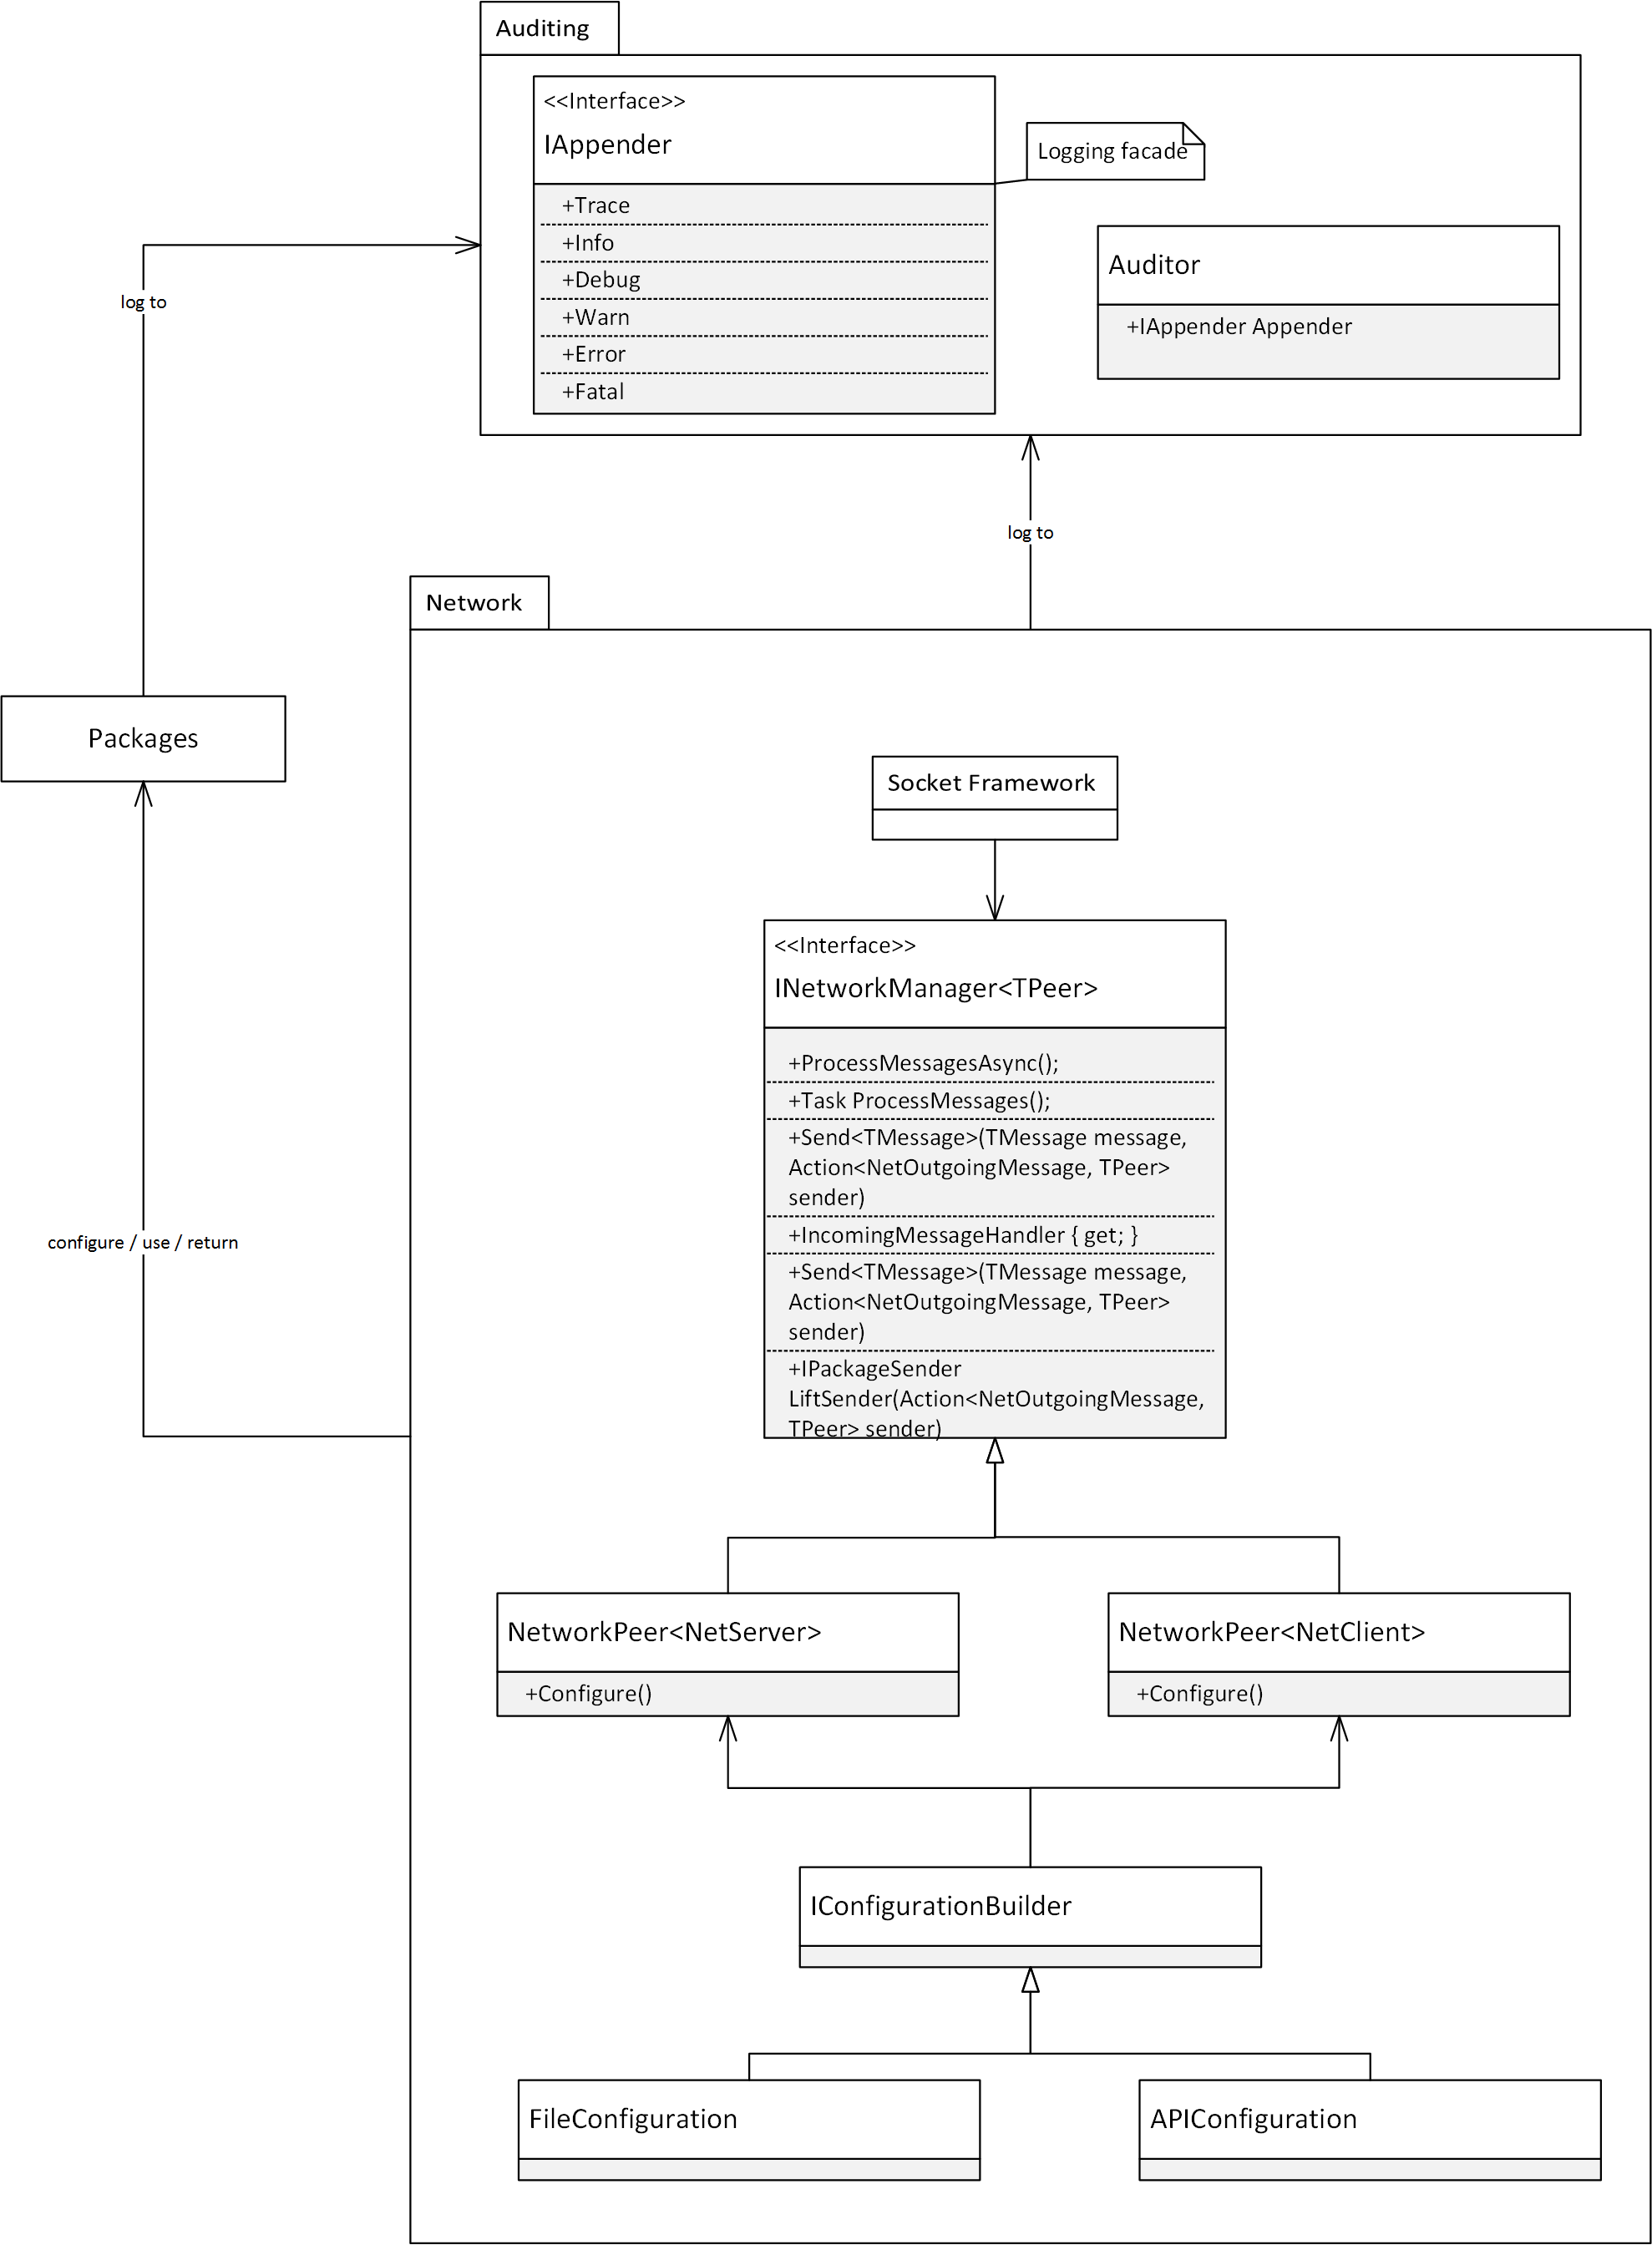
\includegraphics[width=165mm]{Images/network_architecture_networking}
				\caption{Networking Module}
				\label{networking_module}
			\end{figure}		
	\newpage
	\subsection{Παραδείγματα}
	Συντομη επισκόπηση του API.
	\begin{itemize}
		\item Κλάσεις που προορίζονται για ανταλλαγή μηνυμάτων
	\lstset
	{
		style=sharpc, 
		caption={Package Attribute}
	}
		\begin{lstlisting}
[GinetPackage]
 //optional
[PackageSerializer(typeof(MyCustomSerializer))]
public class MyPackage
{
    public string Message { get; set; }
}          
		\end{lstlisting}
		\item Ρύθμιση server
	\lstset
	{
		style=sharpc, 
		caption={Ρύθμιση server}
	}
		\begin{lstlisting}     
var server = new NetworkServer("MyServer",
builder =>
{
	//via reflection
	builder.RegisterPackages(
		Assembly.Load("Packages.Assembly.Name"));
	//or manually
	builder.RegisterPackage<MyPackage>();
}
cfg =>
{
	cfg.Port = 1234;
	cfg.ConnectionTimeout = 5.0f;
	cfg.MaxConnections = 10;
	//Additional configuration
}
//optional, logging output, default is the one supplied			 
out: new ActionAppender(Console.WriteLine) 
		\end{lstlisting}
		\item Καταγραφή κινήσεων		
	\lstset
	{
		style=sharpc, 
		caption={Καταγραφή κινήσεων}
	}
		\begin{lstlisting}
server.IncomingMessageHandler.LogTraffic();
		\end{lstlisting}		
		\item Απάντηση κατά την παραλαβή μηνύματος
	\lstset
	{
		style=sharpc, 
		caption={Απάντηση κατά την παραλαβή μηνύματος}
	}
		\begin{lstlisting}
server.Broadcast<ChatMessage>((msg, im, om) =>
{
	server.Out.Info($"Received {msg.Message}");
	server.SendToAllExcept(om, im.SenderConnection, NetDeliveryMethod.ReliableOrdered, channel: 0);
}, 
packageTransformer: msg => 
msg.Message += "this is broadcasted");	


server.BroadcastExceptSender<ChatMessage>((sender, msg) =>
{
	server.Out.Info($"Broadcasting {msg.Message}. Received from: {sender}");
});
		\end{lstlisting} 		

		\item Κώδικας ο οποίος εκτελείται κατά την παραλαβή συγκεκριμένου τύπου μηνύματος
	\lstset
	{
		style=sharpc, 
		caption={Incoming type handler}
	}
		\begin{lstlisting}
server.IncomingMessageHandler.OnMessage(
	NetIncomingMessageType.ConnectionApproval, 
	incomingMsg =>
{
	//Configure connection approval
	var parsedMsg = server
		.ReadAs<ConnectionApprovalMessage>(incomingMsg);
	if(parsedMsg.Password ==
		 "my secret and encrypted password")
	{
		incomingMsg.SenderConnection.Approve();
		incomingMsg.SenderConnection.Tag = 
			parsedMsg.Sender;
	}
	else
	{
		incomingMsg.SenderConnection.Deny();
	}
});
		\end{lstlisting}
		\item Εκτελέσιμος κώδικας κατά την παραλαβή συγκεκριμένου μηνύματος-κλάσης
	\lstset
	{
		style=sharpc, 
		caption={Incoming message handler}
	}
		\begin{lstlisting}
server.IncomingMessageHandler
.OnPackage<MyPackage>((msg, sender) => 
	Console.WriteLine(
	$"{msg.Message} from {sender.SenderConnection}"));
		\end{lstlisting}	
		\item Αποστολή μηνύματος-κλάσης
		\lstset{style=sharpc}
		\begin{lstlisting}
server.Send(
	new MyPackage { Message = "Hello" },
(outgoingMessage,peer) => 
	peer.SendMessage(outgoingMessage,
		NetDeliveryMethod.ReliableOrdered);
		\end{lstlisting}		
		\item Lift αποστολής μηνύματος
	\lstset
	{
		style=sharpc, 
		caption={Message sender lift}
	}
		\begin{lstlisting}
var packageSender = client.LiftSender((msg, peer) =>
	peer.SendMessage(msg, 
		NetDeliveryMethod.ReliableOrdered));
		
packageSender.Send(new MyPackage { Message = "Hello" });	
		\end{lstlisting}	
		\item Διαγραφή handler
	\lstset
	{
		style=sharpc, 
		caption={Διαγραφή handler}
	}
		\begin{lstlisting}	
var handlerDisposable = server.IncomingMessageHandler
	.OnPackage<MyPackage>((msg, sender) => {}));
		
handlerDisposable.Dispose();	
		\end{lstlisting}		
		\item Η ρύθμιση και το API του client είναι πανομοιότυπo με του server. Στη θέση του \textit{NetworkServer} χρησιμοποιείται ο \textit{NetworkClient} όπου και τα δύο υλοποιούν τον \textit{NetworkManager<TPeer> where TPeer:NetPeer}		
	\end{itemize}
	
	\section{Testing}
	Μια καλή αρχιτεκονική υποστηρίζεται από την ευκολία της δοκιμαστικότητας ανά μονάδα (unit testability). Το framework χρησιμοποιεί functional τεχνικές, οι οποίες εύκολα μπορούν να αντικατασταθούν με mocks. Ο χρήστης μπορεί να απομιμήσει την παραλαβή ή αποστολή πακέτων και να ενημερώνει την μονάδα επεξεργασίας μηνυμάτων από το τρέχων thread.
	
	\lstset
	{
		style=sharpc, 
		caption={Incoming Package Handler}
	}
	\begin{lstlisting}
	
[TestMethod]
public void Incoming_Package_GetsHandled()
{
	//Arrange
	var client = new NetworkCliient(
		builder => 
			builder.Register<MyPackage>(),
		cfg=> {});
		
	var mockedHandler = 
		new Mock<Func<MyPackage,NetIncomingMessage>>();
	mockedHandler.Setup( x => 
		x(It.IsAny<MyPackage>()));
	
	client
	.IncomingMessageHandler
	.OnPackage<MyPackage>(mockedHandler);	
	
	//Act	
	client.IncomingMessageHandler.SimulateReceive(
		new MyPackage());	
	client.ProcessMessages().RunSynchronously();
	
	//Assert
	mockedHandler.Verify(x=>x(), Times.Once()));
}
	\end{lstlisting}
		
	Επίσης παρέχεται η δυνατότητα της προσομοίωσης χαμένων πακέτων, για να δοκιμαστεί πως η εφαρμογή ανταποκρίνεται σε περιβαλλον κακής διαδικτύωσης και να αναπτυχθούν τεχνικές network prediction για εξομάλυνση της κίνησης.
	